\chapter{Empirical evaluation of compression algorithms}
In this chapter, we compare lossless and lossy algorithms in terms of compression performance using both real and 
generated time series data. The lossless compression algorithms that we have chosen are Gorilla, LZ4,
Deflate and Zstandard. For the lossy algorithm part, we take a look at how PCM and PLA perform against each other.

\section{Datasets}
For these benchmarks, we have used three different datasets. The first dataset was generated from the
Time Series Benchmark Suite, a project mantained by TimescaleDB \cite{timescale_2019_timescaletsbs}.
The second dataset was provided by Dynatrace. Dynatrace is a Software Intelligence platform with a strong
emphasis on application performance monitoring. The datasets consist of metrics gathered from
different hosts running a wide range of applications under different loads.
The metrics we have chosen to collect are the following:
\begin{itemize}
    \item Host CPU Usage: Percentage of overall CPU usage
    \item Host CPU System: Percentage of CPU time used by the kernel
    \item Host CPU User: Percentage of CPU time used by user space processes
    \item Host CPU Io Wait: Percentage of CPU time spent waiting for input/output operations
    \item Host Memory Used: Percentage of memory used
    \item Host Memory Usage: Memory usage in bytes
    \item Host Disk Read Time: Disk read time in milliseconds
    \item Host Disk Write Time: Disk write time in milliseconds
\end{itemize}
The third dataset was provided by the New York Taxi and Limousine Commisson (TLC), and it constists
of records representing taxi trips, including information such as duration of the trip, amount
charged, tip amount \cite{tlc2019_dataset}.

\section{Methodology}
We have created a Java project which receives data from the standard input, and, after
compressing the data, returns statistics such as initial data size, compressed data size and
the compression ratio. The code is available on github \cite{dovidio_2019_dovidiotscompressionthesis}.
We had to take into account how the datasets we receive in input can have different formats,
for this reason we implemented different serializer.
For gorilla compression, we have used an open source java implementation of the algorithm
\cite{burmanm_2018_burmanmgorillatsc}. Deflate, on the other hand, is already present in the the package
\textit{java.util.zip}, using the zlib library under the hood \cite{a2019_deflater}.
For LZ4 and ZStandard we have used open source implementations \cite{lz4_2019_lz4lz4java}\cite{luben_2015_lubenzstdjni}.
To run the project one must run the following lines
\lstset{
    basicstyle=\small,
    stringstyle=\ttfamily
}
\begin{lstlisting}[language=bash]
  $ ./gradlew shadowJar
  $ java -jar
  TimeseriesCompressionBenchmarks-all.jar [format] [algorithm]
\end{lstlisting}
where format specify the format of the input files and can assume the following values: devops, dynatrace, taxi.
Algorithm specifies instead which compression algorithm we want to run and can be gorilla, lz4, deflate, zstandard.

\section{Lossless algorithms and generated data}
Figure~\ref{devops_lossless_compression} illustrates the result of applying different compression algorithms
with generated data. It clearly shows how Gorilla is outperforming the other lossless compression algorithms.

\begin{figure}[!htbp]
\begin{center}
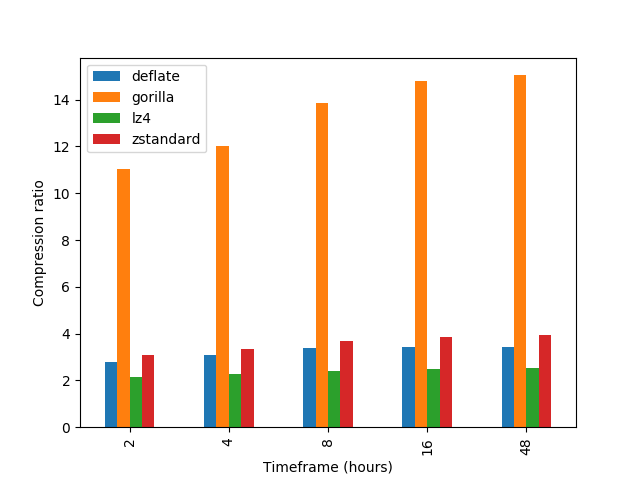
\includegraphics[width=300pt]{devops_bar_chart}
\caption[compression]{Data compressed with Gorilla, Deflate, ZStandard, LZ4. Higher values indicates higher compression ratios.}
\label{devops_lossless_compression}
\end{center}
\end{figure}

\section{Comparing lossless algorithms}
For the lossless algorithms, we have chosen to evaluate Gorilla performance against general-purpose
algorithms with generated and real-time series data. The metric in which we are interested is the
compression ratio, while we don't evaluate compression speed as this is dependent of the implementations we have
chosen. We have created a Java program that reads data from the input stream and returns the compression ratio
achieved by the algorithm selected. We decided to use Java because we could easily find implementations for
all the algorithms listed above. The program requires to specify the format of the dataset provided and the
algorithm to use for compression.

\section{Comparing lossy algorithms}
The lossy algorithms we have decided to compare are Piecewise Constant Approximation and Piecewise Linear
Approximation. Both algorithms were implemented by us in Java. We have used the same datasets as the one used
for the lossless algorithms


